% NOTE (2026-09-25): superseded by ../draft.tex, which was revised after a 46-item review; this file is kept as a source only.
% =====================================================================================
% sections/data_results.tex -- Data and measurement, and Results, of the short draft of "Degrees of Separation"
% (author: Sora Yng). Written 2026-09-25 for \input; no preamble. Terminology follows theory_core.tex: field rank F,
% university-wide rank G, coupling, intake selectivity, programme.
% Needs graphicx, booktabs, array, amsmath and natbib. Figures are reused from outputs/figures; the paths assume the
% including file is compiled in paper/short/. Citation keys: ../refs_merged.bib only.
% Cross-references: sec:thy (theory_core.tex); cor:thy-onefactor (theory_appendix.tex). No proposition label is
% referenced, because theory_core.tex is being revised in parallel.
% "SI S3"--"SI S7" point to the sections of paper/si.tex (S3 coupling, S4 selectivity, S5 UK, S6 career, S7 licensing).
% Every number is copied from paper/main.tex (Sections 4-5, Tables 1-3) or paper/si.tex (S3 per-field table, S5);
% none is new. Sources of the less obvious ones:
%   +0.71 CS, +0.69 economics, +0.07 nursing, +0.04 music ... si.tex, per-field table (tab:fields)
%   I^2 = 0.69; +0.68 [+0.54, +0.82]; +0.94 (23 fields) ...... main.tex sec:map; si.tex sec:crosssource, sec:ordering
%   0.173 vs 0.076 Shapley shares; c_F - c_G ................. main.tex sec:status ("Department prestige against ...")
%   15 of 57 fields (c_F > c_G) ................................ main.tex sec:status; THEORY_NOTES.md section 4
%   85% [80, 90]; 73% [67, 78]; 66% [51, 79] .................. main.tex sec:uk; si.tex sec:ukcontrols, sec:ukrobust
%   0.39 of the raw slope; +0.0305 -> +0.0103 ................. main.tex sec:career
%   +0.120 vs +0.523, -0.404 [-0.566, -0.238]; +0.570; +0.55 . main.tex sec:boundary; si.tex sec:ukpayscale
%   T0, T1, T7, T8 verdicts ................................... main.tex sec:prestige, sec:map; THEORY_NOTES.md section 13
% =====================================================================================
\providecommand{\ci}[2]{$[#1,\allowbreak\,#2]$}

\section{Data and measurement}\label{sec:data}

All inputs are public and are listed in Table~\ref{tab:data} with the samples used. The academic market's
ordering is the published SpringRank hiring rank of \citet{wapman2022quantifying}, from a census of faculty at 368
PhD-granting US institutions in 2011--2020 \citep{wapman2022data}. We use its field rank $F_{if}$ and its
university-wide rank $G_i$, signed so that higher values mean higher standing. The graduate market's ordering is
the median earnings $Y$ of each programme's bachelor's graduates. In the US these are College Scorecard medians four
years after completion \citep{scorecard} and PSEO medians one, five and ten years after graduation for fixed
cohorts \citep{pseo, pseo2026}. In the UK they are LEO medians, which are also released by graduates' prior
attainment \citep{dfe_leo_provider}. The UK has no field rank; its $G$ is a SpringRank of PhD-to-faculty moves in
ORCID-derived records \citep{li2026orcid}. Intake selectivity is mean SAT and admission rate in the US, and the
share of graduates with 360 or more UCAS points in the UK. Coupling is the Spearman correlation, across the
institutions that teach a field, between $F$ (UK: $G$) and $Y$. Partial coupling correlates the rank residuals of
both after regressing them on the ranks of the controls. The reliability of $F$ lies between 0.81 (lower bound)
and 0.96 (extrapolated), and that of $G$ is 0.99. Brackets are 95\% intervals that resample or cluster by
institution; UK intervals resample subjects and then providers. Two tests (specified before the analysis; not
publicly registered) qualify $F$: it partly reflects doctoral production (T0), and it orders departments
differently as placers and as hirers of PhDs (T1). Pay includes intake selection and where graduates work:
five-year coupling is unchanged net of destination wage levels (T7), but about a fifth of it runs between employer
sectors (T8).

\begin{table}[!tbp]
\centering
\caption{Data. All sources are public; versions and access dates are recorded in the repository.}\label{tab:data}
\footnotesize
\setlength{\tabcolsep}{3pt}
\begin{tabular}{@{}>{\raggedright\arraybackslash}p{0.22\linewidth}>{\raggedright\arraybackslash}p{0.30\linewidth}>{\raggedright\arraybackslash}p{0.28\linewidth}>{\raggedright\arraybackslash}p{0.14\linewidth}@{}}
\toprule
Source & Measure & Sample used & Role \\
\midrule
Faculty hiring \citep{wapman2022data} & published SpringRank ranks, hires 2011--2020 & 66 fields; 52 with $\ge15$
matched institutions & $F$, $G$ (US) \\
College Scorecard \citep{scorecard} & median earnings of bachelor's completers four years after completion; June 2026
release & 3,444 programmes in 52 fields & $Y$ (US) \\
Scorecard institution files & mean SAT, admission rate, Pell share, control & 46--47 fields &
selectivity (US) \\
PSEO \citep{pseo, pseo2026} & median earnings one, five and ten years after graduation; releases V4.13.0, V4.14.1
& fixed cohorts 2001--03 to 2010--12; 39 fields, 106 institutions & $Y(t)$ (US) \\
DfE LEO \citep{dfe_leo_provider} & median earnings one, three and five years after graduation, also by
prior-attainment band & cohorts 2013/14--2016/17; 33 subjects, 134 providers & $Y(t)$, selectivity (UK) \\
ORCID-derived records \citep{li2026orcid} & PhD-to-faculty moves within Great Britain & 11,987 moves & $G$ (UK) \\
\bottomrule
\end{tabular}
\end{table}

% =====================================================================================
\section{Results}\label{sec:results}

Each result compares orderings of the same institutions; Section~\ref{sec:thy} states when those orderings read as
the two markets' valuations.

\subsection{The two orderings agree, to a degree that varies across fields}\label{sec:res-map}

In most fields, the academic market and the graduate market order the same programmes alike. Across the 52 fields
with at least 15 matched institutions, mean coupling of $F$ with four-year pay is $+0.419$ \ci{+0.355}{+0.482}
(Fig.~\ref{fig:map}). Coupling lies more than 1.96 bootstrap standard errors above zero in 39 fields and below zero
in none. It is $+0.71$ in computer science and $+0.69$ in economics, but $+0.07$ in nursing and $+0.04$ in music.

Fields differ by more than institution sampling produces: in a three-level meta-analytic model of 57 fields,
$I^2=0.69$ \citep{konstantopoulos2011fixed, higgins2002quantifying}. Noise in the programme medians accounts for
part of this spread (SI~S3). The field ordering recurs on PSEO five-year pay, whose field couplings correlate with
Scorecard's at $+0.68$ \ci{+0.54}{+0.82} (57 fields). Both sources use $F$ and share many institutions, so this is
robustness to the earnings measure, not an independent replication. The ordering also follows how steeply each
field's pay rises with mean SAT, at a true-score correlation of $+0.94$ (23 fields). One university factor, priced
differently by field, would produce this collinearity (Corollary~\ref{cor:thy-onefactor}). The field map therefore
cannot separate a department gradient in pay from a gradient in university status.

\begin{figure}[!tbp]
\centering
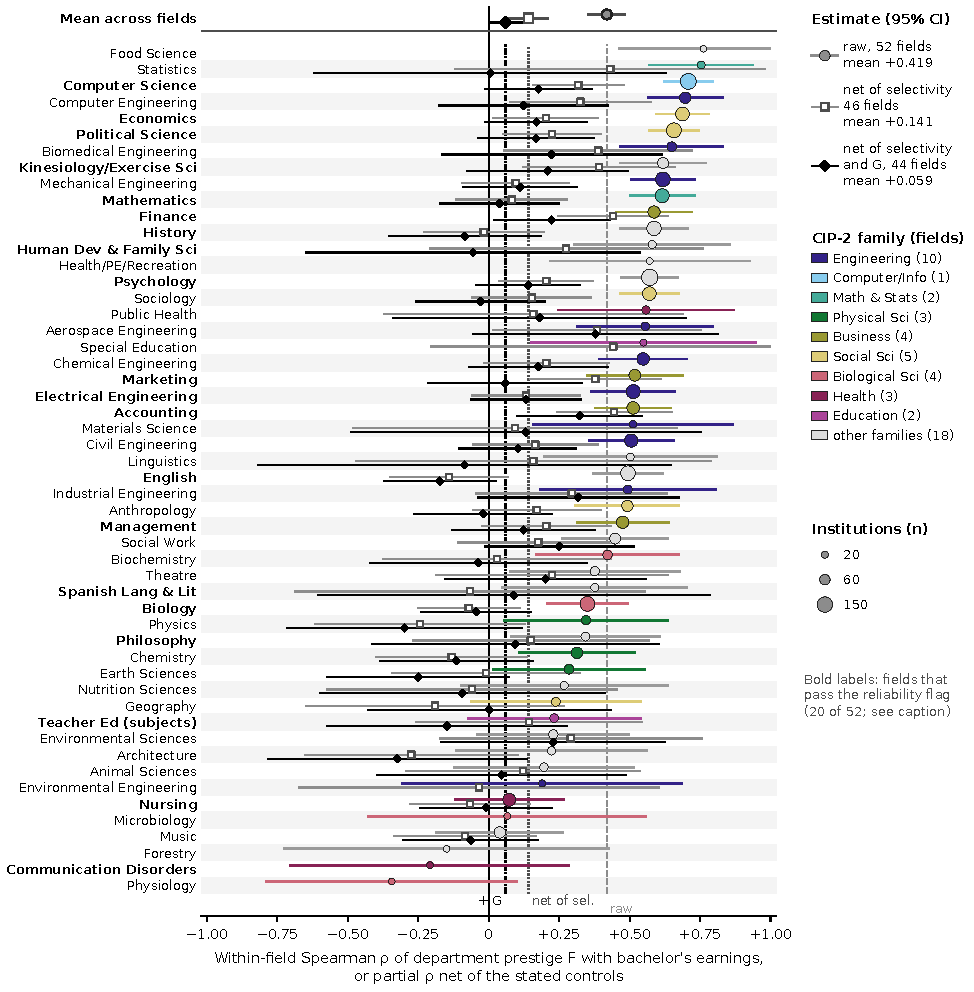
\includegraphics[width=0.86\linewidth]{../../outputs/figures/paper_fig1.pdf}
\caption{Coupling by US field. Spearman correlation across institutions between the field rank $F$ (``department
prestige'' in the axis label) and Scorecard median pay four years after completion, for the 52 fields with at
least 15 matched institutions. Circles: raw coupling, coloured by CIP-2 family and sized by institutions. Squares:
partial coupling net of mean SAT, admission rate, Pell share, control and state earnings level (46 fields).
Diamonds: net of $G$ as well (44 fields). Bars: $\pm1.96$ institution-bootstrap standard errors, cut at $\pm1$; top
row: means with 95\% intervals. Bold labels: the 20 fields whose earnings pass a reliability flag (SI~S3); the flag
does not certify precision.}\label{fig:map}
\end{figure}

\subsection{Agreement sits at the university and is largely shared with intake selectivity}\label{sec:res-name}

Most of the agreement in the US is shared with intake selectivity. Pell share, control and state earnings level
lower mean coupling from $+0.43$ to $+0.31$, and adding admission rate and mean SAT lowers it to $+0.14$ (44 fields;
Fig.~\ref{fig:status}a). The split between these steps depends on the order in which controls enter. On the 46
fields estimable with all five controls, mean partial coupling is $+0.141$ \ci{+0.075}{+0.208}. Dating the controls
to graduates' entry years leaves it where it was (SI~S4). In per-field rank regressions, selectivity takes a mean
Shapley share of $R^2$ of 0.173, against 0.076 for $F$ (Fig.~\ref{fig:status}c). Mean SAT can proxy what a
university provides as well as whom it admits \citep{dale2002estimating}. The fall therefore measures what public
data cannot separate from intake, not what selectivity causes.

The agreement sits at the university level rather than the department. Before any control, $G$ couples with a
field's pay slightly more strongly than $F$ does: the mean difference of the two couplings is $c_F-c_G=-0.049$
\ci{-0.085}{-0.011} (57 fields; Fig.~\ref{fig:status}d). In only 15 of these 57 fields does $F$ couple more strongly
than $G$. Under either reliability correction, and net of selectivity, $F$ does not detectably out-predict $G$. Net
of the five controls and $G$, mean coupling is $+0.059$ \ci{+0.003}{+0.114} (44 fields), and across ten such
specifications its interval excludes zero in four.

Within institutions, the part of agreement specific to the department is small. Institution fixed effects absorb
what is common to a university's programmes, including location. With field-specific slopes on mean SAT, admission
rate, Pell share and $G$, one within-field standard deviation (SD) of $F$ goes with 0.84\% higher four-year pay. The
slope is $+0.0084$ \ci{+0.0000}{+0.0164} across 2,889 programmes, 168 institutions and 47 fields
(Fig.~\ref{fig:status}b). The interval reaches zero, and with one- and five-year medians, which describe other
cohorts, the slope is about zero. Corrected for error in $F$, the slope is about 3\% at the lower-bound reliability.
The department part is thus diluted, not shown to be absent.

Only computer science has an individually clear remainder: $+0.050$ log points per SD of $F$ \ci{+0.012}{+0.096},
pooled over horizons (128 programmes). Its sample lacks 21 of the 50 highest-ranked computer-science departments,
among them the University of California campuses. There, too, the data cannot separate selection into the major
\citep{bleemer2022will} from department standing (SI~S4).

\begin{figure}[!tbp]
\centering
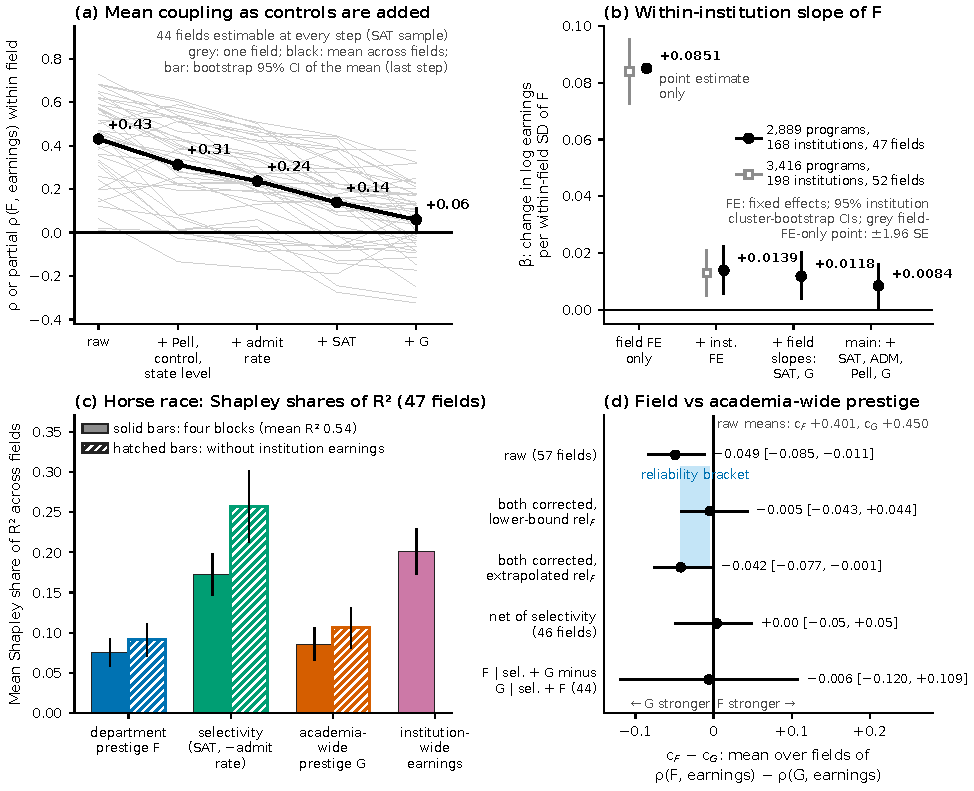
\includegraphics[width=\linewidth]{../../outputs/figures/paper_fig2.pdf}
\caption{What remains of US coupling after university-level controls (Scorecard, four-year pay). The panels label
$F$ ``department prestige'' and $G$ ``academia-wide prestige''. (a) Mean coupling as controls are added (44 fields;
grey lines: single fields). (b) Within-institution slope of log pay per within-field SD of $F$, from field fixed
effects alone to the main specification, which adds institution fixed effects and field-specific slopes on mean
SAT, admission rate, Pell share and $G$. (c) Mean Shapley shares of $R^2$ in per-field rank regressions (47
fields), with and without (hatched) institution-wide earnings. (d) Mean difference $c_F-c_G$ between the couplings
of $F$ and $G$: raw, corrected for error in $F$ at either reliability, and net of selectivity. 95\%
institution-bootstrap intervals.}\label{fig:status}
\end{figure}

\subsection{In the UK, most agreement survives a direct prior-attainment control}\label{sec:res-uk}

The UK data add what the US data lack: pay by graduates' own prior attainment. They have no field rank, so they
bear on the university level only. Coupling of $G$ with five-year pay averages $+0.486$ \ci{+0.398}{+0.559} across
33 subjects, close to the US coupling of $G$ with Scorecard pay ($+0.450$, 57 fields). Standardising each
provider's pay for its mix of attainment bands, with band gradients measured within providers, leaves 85\%
\ci{80}{90} of the rank coupling (32 subjects; Fig.~\ref{fig:uk}a,b). Less survives in pay terms: 73\%
\ci{67}{78} of the log-earnings gradient in $G$. Comparing same-band graduates across providers keeps 66\%
\ci{51}{79}, a share lowered by noise in the band medians. Bands are coarse, so sorting within a band is not
controlled, and that pushes every share up (SI~S5).

What survives tracks intake selectivity at least as closely as $G$. Among graduates of the same attainment band,
selectivity keeps a partial coupling of $+0.252$ \ci{+0.172}{+0.310} net of $G$. Net of selectivity, $G$ keeps
$+0.033$, which is not distinguishable from zero (28 subjects; Fig.~\ref{fig:uk}c). The UK $G$ may carry error: at
a validity of 0.74, the data allow its same-band partial to reach $+0.26$ (SI~S5). Selectivity is itself a status
measure, so this does not show that status is unrelated to pay. With a hiring-network rank, the pattern matches
the one \citet{britton2022how} report for league tables.

\begin{figure}[!tbp]
\centering
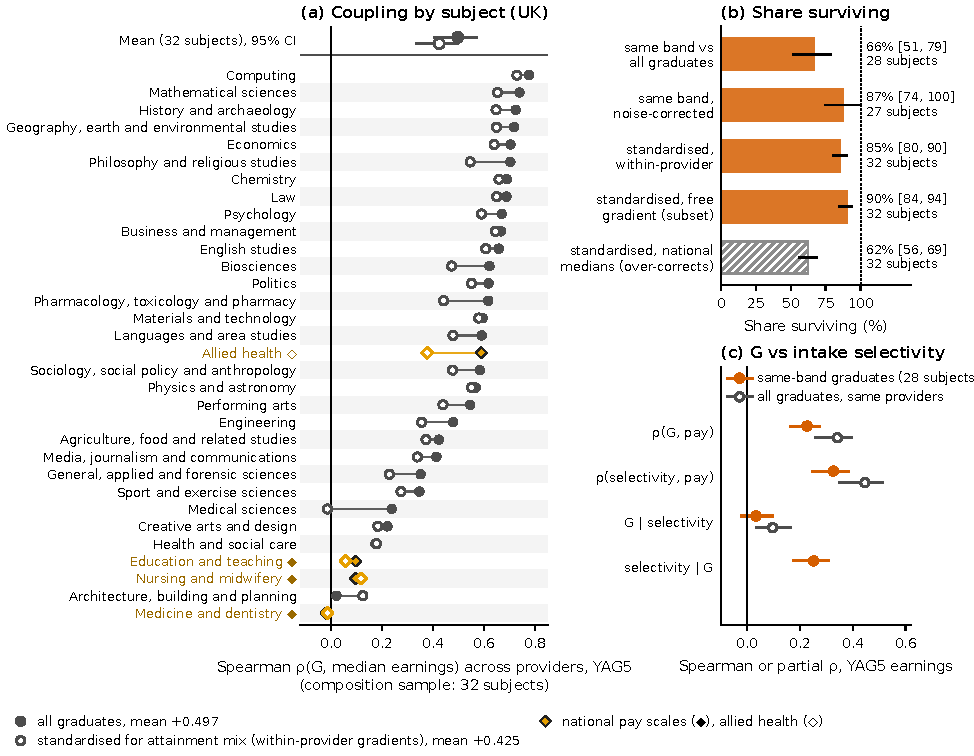
\includegraphics[width=\linewidth]{../../outputs/figures/paper_fig3.pdf}
\caption{UK coupling and prior attainment (LEO five-year pay, cohorts 2013/14--2016/17). (a) Coupling of $G$ by
subject for all graduates (filled) and standardised for attainment mix (open), on the 32-subject composition sample,
whose values differ slightly from those on all providers quoted in the text. Diamonds: the three subjects paid on
national scales; open diamond: allied health. (b) Share of coupling surviving each attainment control; national
band medians over-correct and give a floor. (c) Coupling of $G$ and of intake selectivity with pay, and each net of
the other, for same-band graduates (triangles) and all graduates of the same providers (circles). Two-stage
bootstrap 95\% intervals over subjects and providers.}\label{fig:uk}
\end{figure}

\subsection{Agreement rises with years since graduation and is weak where pay follows a schedule}\label{sec:res-time}

Within fixed graduation cohorts, coupling rises with years since graduation in both countries (SI~S5, S6). In the
US it goes from $+0.173$ one year after graduation to $+0.451$ at ten years (39 fields; PSEO), a mean per-field
slope of $+0.031$ \ci{+0.021}{+0.041} per year. In the UK it goes from $+0.379$ at one year to $+0.484$ at five, or
$+0.026$ \ci{+0.014}{+0.037} per year (33 subjects). A within-cohort change mixes career time with calendar time, so
the career part can only be bounded. If calendar and cohort trends are both non-negative, the US career-time slope
lies between $+0.015$ and $+0.031$ per year \citep{fosse2019bounding}.

About three fifths of the US rise is shared with selectivity, and graduate study is not excluded. Net of
entry-year mean SAT and admission rate, the slope keeps 0.39 of its raw size (109 field-by-cohort cells). If
graduates of higher-ranked universities more often leave the earnings data to study and return with higher pay,
coupling would rise mechanically. Controlling for coverage and the university's research-doctorate rate lowers the
slope from $+0.0305$ to $+0.0103$ per year. That rate tracks $G$, however, so the drop mixes the timing of study
with status (SI~S6).

Coupling is weak where most graduates are paid on a national schedule. In the UK, nursing and midwifery, medicine
and dentistry, and education and teaching couple at $+0.120$, against $+0.523$ for the other 30 subjects
(difference $-0.404$ \ci{-0.566}{-0.238}; Fig.~\ref{fig:uk}a). The gap persists after standardising each
provider's pay for its attainment mix (SI~S5). Allied health, much of it also paid on national bands, is an
exception at $+0.570$, as is US special education ($+0.55$), paid mostly on district salary schedules. Where a
schedule sets pay, pay does not reveal employers' valuation, so weak coupling there is not evidence that employers
order universities differently (Section~\ref{sec:thy}). In the US, the association of $F$ with pay net of region
falls with the share of a field's graduates in strictly licensed occupations. That contrast lies between
discipline families, however, and is fragile (SI~S7).
